%   %==========================================================================
%   %  Section : ベクトルの性質
%   %==========================================================================
        %==================================================================
        %  SubSection
        %==================================================================
            \subsection{ベクトルの内積(図形的)}\label{subsec:VecNaisekiFig}
                ベクトルの内積について,簡単に説明をしておこう.

                2つの任意のベクトルを用意し,$\ba$,$\bb$ とする.ベクトルの \textbf{内積} は
                この2つのベクトルより定義される.
                内積の表し方は,$(\ba\,,\;\bb)$ または $\ba\cdot\bb$ などの複数の表現がある.
                このノートでは,$\ba\cdot\bb$ を内積の記号として使うことにする.
                ベクトルの内積を,次のように,平面図形的に定義する.
                    \\
                    \begin{itembox}[l]{\textbf{ベクトルの内積(図形的)}}
                        \begin{dfn}
                            任意の2つのベクトル $\ba$ と $\bb$ の間に,演算 $\cdot$ を
                            以下のように定義する.
                            \begin{align}
                                 \ba\cdot\bb := | \ba |  | \bb | \cos\theta
                            \end{align}
                            この演算を,ベクトル $\ba$ と $\bb$ の \textbf{内積} という.
                        \end{dfn}
                    \end{itembox}
                    \\

                この式のイメージは,「$\ba$ の $\bb$ 方向の成分の大きさ」と,$\bb$ の積の大きさである.
                    \begin{equation*}
                        \ba\cdot\bb = ( | \ba | \cos\theta ) | \bb |
                    \end{equation*}
                と書いたらイメージしやすい.$| \ba | \cos\theta$ の $|\bb|$ 倍ということである.

                    \begin{figure}[hbt]
                        \begin{center}
                            \includegraphicsdefault{bekutoru_no_naiseki.pdf}
                            \caption{内積}
                            \label{fig:bekutoru_no_naiseki}
                        \end{center}
                    \end{figure}

                例えば,$\theta = 60{}^{\circ}$,$| \ba | = 3$,$| \bb | = 5$ のとき,
                    \begin{align*}
                        \ba\cdot\bb     &= | \ba |  | \bb | \cos\theta = 3 \times 5 \times \cos(60{}^{\circ}) \\
                                            &= 3 \times 5 \times \frac{1}{2} \\
                                            &= \frac{15}{2}
                    \end{align*}
                となる.
        %==================================================================
        %  SubSection
        %==================================================================
            \subsection{ベクトルの内積(代数的)}\label{subsec:VecNaisekiArg}
                実は,ベクトルの内積には,もう一つ別の定義がある.もちろん,上に説明した平面図形的定義と
                全く矛盾しない.別の定義とは,ベクトルの成分に着目した,代数的定義である
                    \footnote{
                        「平面図形的定義」と「代数的定義」は私の造語.
                    }.

                ベクトルの内積の代数的定義は,次式で定義される.
                    \\
                    \begin{itembox}[l]{\textbf{ベクトルの内積(代数的)}}
                        \begin{dfn}
                            任意の2つのベクトル $\ba$ と $\bb$ があるとする.
                            ベクトルの成分を
                                $\ba=\left[\,a_{1},\,a_{2},\,\cdots,\,a_{n}\,\right]$,
                                $\bb=\left[\,b_{1},\,b_{2},\,\cdots,\,b_{n}\,\right]$ で
                            表すとき,この2つのベクトルの間の演算 $\cdot$ を
                            次で定義する
                                \begin{align}
                                    \ba\cdot\bb = \sum_{i=1}^{n} a_{i}b_{i}.
                                \end{align}
                        \end{dfn}
                    \end{itembox}
                    \begin{description}
                        \item[例] 仮に,2つのベクトルの成分は2つとしよう.
                        つまり,$\ba=\left[a_{1},\,a_{2}\right]$,
                                $\bb=\left[b_{1},\,b_{2}\right]$ と仮定する.
                        このときベクトルの内積は
                            \begin{align}
                                \ba\cdot\bb = a_{1}b_{1}+a_{2}b_{2}
                            \end{align}
                        である.
                    \end{description}



        %==================================================================
        %  SubSection
        %==================================================================
            \subsection{図形的内積と代数的内積の関係}
                図形的定義による内積と代数的定義による内積が全く同じことであることは,次のように説
                明できる
                    \footnote{
                        互いに矛盾する定義だったら,内積の定義としてどちらを採用するかを検討しない
                        といけない.もしくは,両方とも採用しないことになるかもしれない.だけど,全
                        く同じことを言っているのだから,都合のよい方を,定義式として採用してよいの
                        である.

                        今回は,まずイメージしやすいように図形的な定義を先に紹介した.
                        だけど,物理学の理論を考えるには,数式で表現する必要がある.
                        $\cos$ 関数を用いた図形的定義でも事足りると思うが,
                        代数的な内積の式も有用なので,紹介をしておいた.
                    }.

                2つの任意のベクトル $\ba$,$\bb$ の内積を考える.
                この2つのベクトルを直交座標の $x$ 座標,$y$ それぞれ座標の成分に分解し,
                    \begin{align*}
                        \begin{cases}
                        \displaystyle \ba = \ba_{x}  +  \ba_{y} \\
                        \displaystyle \ba = \bb_{x}  +  \bb_{y}
                        \end{cases}
                    \end{align*}
                とする.
                    \begin{figure}[hbt]
                        \begin{center}
                            \includegraphicslarge{naiseki_zahyou_zukei.pdf}
                            \caption{内積(代数的定義と図形的定義の関係)}
                            \label{fig:naiseki_zahyou_zukei}
                        \end{center}
                    \end{figure}
                ここで, $\ba$,$\bb$ の内積を図形的に計算してみよう.
                    \begin{align*}
                        \ba\cdot\bb &= ( \ba_{x}  +  \ba_{y} ) \cdot  ( \bb_{x}  +  \bb_{y} ) \\
                                        &= \ba_{x}\cdot\bb_{x} + \ba_{x}\cdot\bb_{y} +\ba_{y}\cdot\bb_{x} + \ba_{y}\cdot\bb_{y}
                    \end{align*}
                右辺の各項を,それぞれ計算しよう.($\cos {0\,}^{\circ}=1$,$\cos {90\,}^{\circ}=0$)
                    \begin{align*}
                        \begin{cases}
                        \displaystyle \ba_{x}\cdot\bb_{x} = |\ba_{x}| |\bb_{x}| \cos {0\,}^{\circ} = a_{x}b_{x}. \\
                        \displaystyle \ba_{x}\cdot\bb_{y} = |\ba_{x}| |\bb_{y}| \cos {90\,}^{\circ} = 0.\\
                        \displaystyle \ba_{y}\cdot\bb_{x} = |\ba_{y}| |\bb_{x}| \cos {90\,}^{\circ} = 0.\\
                        \displaystyle \ba_{y}\cdot\bb_{y} = |\ba_{y}| |\bb_{y}| \cos {0\,}^{\circ} = a_{y}b_{y}.\\
                        \end{cases}
                    \end{align*}
                つまり,
                    \begin{align}
                         \ba\cdot\bb = a_{x}b_{x} + a_{y}b_{y}
                    \end{align}
                である.これで,代数的定義は,図形的定義と同じこだと,分かるだろう.
                    \\
                    \begin{itembox}[l]{\textbf{ベクトルの内積}}
                        直交座標上における,
                        2つの二次元ベクトル $\ba = \left[a_{x} ,\,a_{y}\right]$,
                        $\bb = \left[b_{x} ,\,b_{y}\right]$ に対して,
                        ベクトルの \textbf{内積} $\ba\cdot\bb$を
                        次式で定義する.
                            \begin{align}
                                \ba \cdot \bb := a_{x}b_{x} + a_{y}b_{y}.
                            \end{align}

                        $n$ 次元ベクトル同士の内積の場合,
                            \begin{align}
                                \ba \cdot \bb := \sum_{i=1}^{n}a_{i}b_{i}.
                            \end{align}
                        と定義する.
                    \end{itembox}
                    \\

        %==================================================================
        %  SubSection
        %==================================================================
            \subsection{ベクトルの内積の性質}\label{subsec:VecNaisekiStt}
                ベクトルの内積は1つのベクトル,つまり,自分自身との内積を
                計算することもできる.図形的に計算すると,
                    \begin{align}
                         \ba\cdot\ba =|\ba| |\ba| \cos{0\,}^{\circ}  = |\ba|^{2} .
                    \end{align}
                である.自分自身との内積は,そのベクトルの大きさの二乗になる.

                まとめておこう.今後のことを考えて,ここでは,
                代数的定義を採用しておこう.そのほうが,ベクトルの次元が任意になったとしても,
                その定義式を簡単にイメージできるからである.

                また,ベクトルの内積を考えることで,ベクトル同士が直交しているか否かを
                知ることができる.ベクトル同士が直交するとき,その角度は,${90\,}^{\circ}$ で
                ある.このとき,$\cos{90\,}^{\circ} =0$ なので,内積も0になる.
                内積が0になる他の条件として,
                交わる角度が ${270\,}^{\circ}$ であること($\cos{270\,}^{\circ} =0$でこの場合も直交している),そして,
                そもそも,少なくともどちらか一方のベクトルが零ベクトル,つまり $\ba = ( 0,\,0,\,0 )$ の場合
                である.それ以外には内積は0にならない.よって,次のように言うことができる.
                    \begin{itemize}
                        \item 零ベクトルでない,2つのベクトルの内積が0の場合,
                        この2つのベクトルは直交している.
                    \end{itemize}
                逆に次もいえる.
                    \begin{itemize}
                        \item 零ベクトルでない,2つのベクトルが直交している場合,
                        この2つのベクトルの内積は0である.
                    \end{itemize}

                以上,2つの性質をまとめよう.\\

                    \begin{itembox}[l]{\textbf{ベクトルの内積の性質}}
                        \begin{enumerate}
                            \item 自分自身との内積は,自分自身の大きさの二乗になる.
                                \begin{align}
                                     \ba\cdot\ba = |\ba|^{2} .
                                \end{align}

                            \item 直交座標上における,零ベクトルでない,
                            2つの二次元ベクトル $\ba =\left[a_{x} ,\,a_{y}\right]$,
                            $\bb = \left[b_{x} ,\,b_{y}\right]$ に対して,
                                \begin{align}
                                    \ba \cdot \bb = 0 \quad  \Leftrightarrow \quad  \ba \perp \bb.
                                \end{align}
                        \end{enumerate}
                    \end{itembox}


        %==================================================================
        %  SubSection
        %==================================================================
            \subsection{ベクトルの外積}\label{subsec:VecGaiseki}
            %==============================================================
            %  SubsubSection
            %==============================================================
                \subsubsection{外積の定義}
                向きが互いに異なる2つのベクトルは,ひとつの平面を張る.
                これは図に描けばすぐに分かる.ベクトルは,向きを変えずに,
                もちろん大きさも変えることなく移動させても,
                定義上,同一のベクトルとみなせる.従って,2つのベクトルが
                存在するとき,この2つのベクトルの始点を1箇所に集めて,ベクト
                ルをくっつけることができる.定義上,このような
                操作をベクトルに施しても,ベクトルが変わったわけではないのだ.
                こう考えれば,2つのベクトルは,3角形を張ることがわかる.
                3角形は平面図形の典型であり,つまり,このような3角形を作る
                2つのベクトルはひとつの平面を張ると言えるのである.
                    \begin{figure}[hbt]
                        \begin{tabular}{cc}
                            \begin{minipage}{0.5\hsize}
                                \begin{center}
                                    \includegraphicsdouble{v2vector01.pdf}

                                    (a) 2つのベクトル
                                    \label{fig:v2vector01}
                                \end{center}
                            \end{minipage}
                            \begin{minipage}{0.5\hsize}
                                \begin{center}
                                    \includegraphicsdouble{v2vector02.pdf}

                                    (b) 始点を揃える
                                    \label{fig:v2vector02}
                                \end{center}
                            \end{minipage}
                        \end{tabular}
                        \caption{2つのベクトルは3角形を作る}
                    \end{figure}


                しかし,私達の暮らす世界は,3つの次元をもっている
                    \footnote{
                        少なくとも,私たちは直感的に,縦$\cdot$横$\cdot$高さの
                        3つの方向を認識している.また,方向3つしかないとも直感
                        的に把握している.当然,物理学もこの直感に従って構成さ
                        れる.ただ,最近「超弦理論(スーパーストリンリングス
                        $\cdot$セオリー;super string theory)」という数学的な
                        匂いの濃い理論が,スポットライトを浴びてきてはいるが.
                    }.
                なので,3次元に広がったベクトルを考えることもできる.今までは,
                平面上に存在するベクトルを考えてきたが,
                ここでは次元を1つ追加して,3次元の空間に想像をふくらませよう.

                3つめの方向をもつベクトルをどうやってつくるか.
                そこで考え出されたのが,ベクトルの \textbf{外積} という
                概念である.考え方は簡単.2つのベクトルに直交するような
                ベクトルを作ればいい.
                    \begin{figure}[hbt]
                        \begin{center}
                            \includegraphicslarge{gaiseki_01.pdf}
                            \caption{外積}
                            \label{fig:gaiseki_01}
                        \end{center}
                    \end{figure}

                そのようなベクトルが仮に存在できたとして,それを $\bc$ と
                表すことにしよう.このとき,既存の2つのベクトルを $\ba$,$\bb$ と
                したなら,次式が成立してなければならない.すなわち,
                    \begin{align*}
                        \ba \cdot \bc &= |\ba||\bc| \cos \frac{\pi}{2} = 0 \\
                        \bb \cdot \bc &= |\bb||\bc| \cos \frac{\pi}{2} = 0
                    \end{align*}
                である.直交しているから,内積が0になっているはずである
                    \footnote{
                        $\cos(\pi/2)=0$ に注意.
                    }.
                ベクトル $\bc$ の成分を $(\,c_{1}\,,c_{2}\,,c_{3}\,)$ としよう.
                $\ba$ と $\bb$ についても同様に,
                それぞれ,$(\,a_{1}\,,a_{2}\,,a_{3}\,)$,
                $(\,b_{1}\,,b_{2}\,,b_{3}\,)$ とする.
                そうすると,上の2つの式は,また,以下のよう書いても同じことである.
                すなわち,
                    \begin{align*}
                        a_{1}c_{1} + a_{2}c_{2} + a_{3}c_{3} &= 0. \\
                        b_{1}c_{1} + b_{2}c_{2} + b_{3}c_{3} &= 0.
                    \end{align*}

                ベクトルの方向については,上の2式が成り立つことがその
                条件であるが,向きについては何も言っていない
                    \footnote{
                        \textbf{「方向」と「向き」の違い}\quad
                        「方向」と「向き」という語彙の違いは,日常生活において,
                        ほとんど区別することなしに使っている.話の流れで意味が理
                        解できるのであるから,そもそも区別することに注意を払う必
                        要はない.しかし,正確には,「方向」と「向き」とは,別の
                        意味を持っている.「方向」とは例えば,“東西の方向”とか,
                        “$x$ 軸の方向”のようにつかう.つまり,「方向を決める」
                        とは,多数ある直線から,1つの直線を決めるということであ
                        る.だから,「方向」という語彙には,“正の向き”とか“負
                        の向き”と言ったことは一切含まれていない.「向き」という
                        のは,要するに,自分のいる場所を基準点として,例えば,左
                        右の方向を考えたとき,右か左かを示すものである.別の例で
                        たとえるなら,数直線があって,その基準点0から見て右側を正
                        の向きとし,他方,基準点0から見て左側を負の向きとするよう
                        なことである.「方向」を決めるとは1つの直線を定めること
                        であり,向きを決めるとは,その直線の上の一点にたって,一
                        方を正,他方を負とすることである(「直線上の任意の一点」
                        は,その直線を2つに切断することは明らかですよね).
                    }.
                そこで,次のように向きを決めてしまおう.すなわち,
                    \begin{description}
                        \item[向きの定義]
                            ベクトル $\ba$ とベクトル $\bb$ から生成する
                            外積 $\bc$ のむきは,\textbf{$\ba$ から $\bb$ に
                            向かって右ねじを右まわし回したときに,ネジが進む向き} を正方向
                            する.これを満たすことを,\textbf{右手系をなす} と
                            いう(「右ねじの法則」なんていう表現が使われることも
                            多い.特に,物理学の多数の教科書で用いられる).
                    \end{description}

                    \begin{figure}[hbt]
                        \begin{center}
                            \includegraphicsdefault{migineji_01.pdf}
                            \caption{右ねじを回して進む方向}
                            \label{fig:migineji_01}
                        \end{center}
                    \end{figure}

                ベクトルにはもうひとつの性質である大きさ
                も考えないといけない.どのような大きさにしようと自由だが,
                最も簡潔に大きさを定めたい.もとの2つのベクトル $\ba$,$\bb$ より,
                この二つのベクトルが張る平行四辺形の面積を,その大きさと
                するのが最も簡単だろう.実際,数学的にもこのような定義が
                なされる.これが最も無理のない定義なのだろう.すると,
                $\bc$ の条件として,次式も加わることになる.
                    \begin{align*}
                        |\bc| &= | \ba || \bb | \sin\theta \\
                        &\Leftrightarrow \quad
                        \sqrt{{c_{1}}^{2}+{c_{2}}^{2}+{c_{3}}^{2}}
                        =
                        \sqrt{{a_{1}}^{2}+{a_{2}}^{2}+{a_{3}}^{2}}
                        \sqrt{{b_{1}}^{2}+{b_{2}}^{2}+{b_{3}}^{2}}
                        \sin\theta
                    \end{align*}

                これで,都合3つの条件式と,向きの定義は揃った.もう一度,まとめて書いておこう.
                    \begin{align*}
                        \begin{cases}
                        \; a_{1}c_{1} + a_{2}c_{2} + a_{3}c_{3} = 0 & \\
                        \; b_{1}c_{1} + b_{2}c_{2} + b_{3}c_{3} = 0 & \\
                        \; \sqrt{{c_{1}}^{2}+{c_{2}}^{2}+{c_{3}}^{2}}
                         = \sqrt{{a_{1}}^{2}+{a_{2}}^{2}+{a_{3}}^{2}}
                                     \sqrt{{b_{1}}^{2}+{b_{2}}^{2}+{b_{3}}^{2}}
                                     \sin\theta & \\
                        \; \mbox{$\ba$,\,$\bb$,\,$\bc$,\,は右手系をなす.(向きの定義)} &
                        \end{cases}
                    \end{align*}

                未知数が $c_{1}$,$c_{2}$,$c_{3}$ と三つなのに対し,
                条件式も同じく3つであり,数式的な条件としては必要十分である
                    \footnote{
                        これで,大きさと方向を定めることができる.
                    }.
                また,ベクトルの向きの定義もした.これで,外積を作る準備が
                整った.あとは,外積を作れるかどうか,言い換えれば,このように
                定義した外積というものが存在可能かどうかを,確認すれば良い.


            %==============================================================
            %  SubsubSection
            %==============================================================
                \subsubsection{外積の成分表示}
                このような3式
                    \footnote{
                        正確には,「3つの式と,向きの定義」と書くべきだけど,
                        向きは人間が勝手に選ぶものなので,数式的に気にするもの
                        ではない.
                    }
                を満たすような $\bc$ は存在するのか.存在するとしたら,
                その成分はどのようになるか.それをこれから考えていこうと思う.それで,
                どうやって求めるかなんだけど,その方法は幾つか思い当たる.
                式をくどくどと計算をして発見的に答えを得る方法もあるけれど,
                それだと少々話が長くなり,計算も面倒くさい.なので,この問題の
                答えはすでに得られていることだから,先に答えを見てしまおう.
                そのほうが早い.

                で,その答えとは,
                    \begin{align*}
                        \bc &= (\,c_{1},\,c_{2},\,c_{3}\,) \\
                            &= (\,
                                    a_{2}b_{3} - a_{3}b_{2},\;
                                    a_{3}b_{1} - a_{1}b_{3},\;
                                    a_{1}b_{2} - a_{2}b_{1}
                                \,)
                    \end{align*}
                である.なにやら複雑な式に見えるが,次のように書くと,
                ある規則がみえてくるだろう.
                    \begin{align}\label{eq:VecGaiseki_Seibun}
                        \bc =
                        \left[
                            \begin{array}{c}
                                c_{1} \\
                                c_{2} \\
                                c_{3} \\
                            \end{array}
                        \right]
                        =
                        \left[
                            \begin{array}{c}
                                a_{2}b_{3} - a_{3}b_{2} \\
                                a_{3}b_{1} - a_{1}b_{3} \\
                                a_{1}b_{2} - a_{2}b_{1} \\
                            \end{array}
                        \right].
                    \end{align}

                $\ba$,$\bb$ の成分の添字を縦方向に意識して眺めると,
                巡回($1 \to 2 \to 3 \to 1$)しているのが見える
                    \footnote{
                        複雑そうに見えるけど,規則さえ分かってしまえば,
                        覚えるのはたやすい.最初の $a_{2}b_{3}$ さえ覚えてしまえば,
                        残りは機械的に記述できる.引く数は添字の数字を入れ替えた
                        ものだし,その他の成分については添字を巡回させればいい.
                    }.
                式(\ref{eq:VecGaiseki_Seibun})は,
                先ほど上げた3つの条件式を必要十分に満たす.

            %==============================================================
            %  SubsubSection
            %==============================================================
                \subsubsection{外積の成分表示の検算}
                式(\ref{eq:VecGaiseki_Seibun})が本当に条件を満たすかどうかを,
                確かめておこう.まず,$\bc \perp \ba$,$\bc \perp \bb$ を
                満たすことを示す.やり方は,単純に条件式に成分を代入して,
                式を整理するだけ.
                    \begin{align*}
                         &a_{1}c_{1} + a_{2}c_{2} + a_{3}c_{3} \\
                         &\qquad=   a_{1}(a_{2}b_{3} - a_{3}b_{2})
                             + a_{2}(a_{3}b_{1} - a_{1}b_{3}) + a_{3}(a_{1}b_{2} - a_{2}b_{1}) \\
                         &\qquad=   a_{1}a_{2}b_{3} - a_{1}a_{3}b_{2}
                             + a_{2}a_{3}b_{1} - a_{2}a_{1}b_{3} + a_{3}a_{1}b_{2} - a_{3}a_{2}b_{1} \\
                         &\qquad= 0.
                    \end{align*}
                もうひとつの式も同じように計算できる.
                    \begin{align*}
                         &b_{1}c_{1} + b_{2}c_{2} + b_{3}c_{3} \\
                         &\qquad=   b_{1}(a_{2}b_{3} - a_{3}b_{2})
                             + b_{2}(a_{3}b_{1} - a_{1}b_{3}) + b_{3}(a_{1}b_{2} - a_{2}b_{1}) \\
                         &\qquad=   b_{1}a_{2}b_{3} - b_{1}a_{3}b_{2}
                             + b_{2}a_{3}b_{1} - b_{2}a_{1}b_{3} + b_{3}a_{1}b_{2} - b_{3}a_{2}b_{1} \\
                         &\qquad= 0.
                    \end{align*}

                たしかに,二つの条件式を満たしている.このことにより,
                ベクトル $\bc$ は,ベクトル $\ba$,$\bb$ に直交している
                ことが確かめられた.つまり,ベクトル $\bc$ の方向は
                条件に沿うものであると言える.

                では,残りの大きさに関する条件式について,それを満たすか
                を計算してみよう.もう一度,大きさを決める条件式を
                書くと,
                    \begin{align*}
                        &\sqrt{{c_{1}}^{2}+{c_{2}}^{2}+{c_{3}}^{2}}
                        =
                        \sqrt{{a_{1}}^{2}+{a_{2}}^{2}+{a_{3}}^{2}}
                        \sqrt{{b_{1}}^{2}+{b_{2}}^{2}+{b_{3}}^{2}}
                        \sin\theta
                    \end{align*}
                でるが,両辺を2乗して,
                    \begin{align*}
                        {c_{1}}^{2}+{c_{2}}^{2}+{c_{3}}^{2}
                        =
                        \left({a_{1}}^{2}+{a_{2}}^{2}+{a_{3}}^{2}\right)
                        \left({b_{1}}^{2}+{b_{2}}^{2}+{b_{3}}^{2}\right)
                        {\sin}^{2}\theta.
                    \end{align*}
                ここで,三角関数の公式 ${\sin}^{2}\theta + {\cos}^{2}\theta = 1$ を
                思い起こし,${\sin}^{2}\theta = 1 - {\cos}^{2}\theta $ と置き換えて,
                    \begin{align*}
                        &{c_{1}}^{2}+{c_{2}}^{2}+{c_{3}}^{2} \\
                        &\quad =    \left({a_{1}}^{2}+{a_{2}}^{2}+{a_{3}}^{2}\right)
                                    \left({b_{1}}^{2}+{b_{2}}^{2}+{b_{3}}^{2}\right)
                                    \left(1 - {\cos}^{2}\theta \right) \\
                        &\quad =    \left({a_{1}}^{2}+{a_{2}}^{2}+{a_{3}}^{2}\right)
                                    \left({b_{1}}^{2}+{b_{2}}^{2}+{b_{3}}^{2}\right) \\
                                    &\quad \qquad -\left({a_{1}}^{2}+{a_{2}}^{2}+{a_{3}}^{2}\right)
                                        \left({b_{1}}^{2}+{b_{2}}^{2}+{b_{3}}^{2}\right)
                                        {\cos}^{2}\theta.
                    \end{align*}
                最後の行の
                    \begin{equation*}
                        \left({a_{1}}^{2}+{a_{2}}^{2}+{a_{3}}^{2}\right)
                        \left({b_{1}}^{2}+{b_{2}}^{2}+{b_{3}}^{2}\right)
                        {\cos}^{2}\theta.
                    \end{equation*}
                に注目すると,
                    \begin{align*}
                        &\left(
                            \sqrt{{a_{1}}^{2}+{a_{2}}^{2}+{a_{3}}^{2}}
                            \sqrt{{b_{1}}^{2}+{b_{2}}^{2}+{b_{3}}^{2}}
                            {\cos}\theta
                        \right)^{2} \\
                            &\qquad=
                            \left(
                                \ba \cdot \bb
                            \right)^{2} \\
                            &\qquad=
                            \left(
                                a_{1}b_{1}+a_{2}b_{2}+a_{3}b_{3}
                            \right)^{2}.
                    \end{align*}

                つまり,大きさの定義式は以下のように書き換えられる.
                    \begin{align*}
                        &{c_{1}}^{2}+{c_{2}}^{2}+{c_{3}}^{2} \\
                        &\qquad =   \left({a_{1}}^{2}+{a_{2}}^{2}+{a_{3}}^{2}\right)
                                    \left({b_{1}}^{2}+{b_{2}}^{2}+{b_{3}}^{2}\right)
                                    \left(1 - {\cos}^{2}\theta \right) \\
                        &\qquad =   \left({a_{1}}^{2}+{a_{2}}^{2}+{a_{3}}^{2}\right)
                                    \left({b_{1}}^{2}+{b_{2}}^{2}+{b_{3}}^{2}\right)
                                    -   \left(
                                            a_{1}b_{1}+a_{2}b_{2}+a_{3}b_{3}
                                        \right)^{2}.
                    \end{align*}

                この式を,ベクトル $\bc$ が満たしていることを確認すればよい.
                    \begin{align*}
                        |\bc|^{2}
                        &=
                        {c_{1}}^{2}+{c_{2}}^{2}+{c_{3}}^{2} \\
                        &=
                         {(a_{2}b_{3} - a_{3}b_{2})}^{2}
                         + {(a_{3}b_{1} - a_{1}b_{3})}^{2}
                         + {(a_{1}b_{2} - a_{2}b_{1})}^{2} \\
                        &=
                        \left(
                            {a_{2}}^{2}{b_{3}}^{2} + {a_{3}}^{2}{b_{2}}^{2} - 2a_{2}a_{3}b_{2}b_{3}
                        \right)
                        + \left(
                            {a_{3}}^{2}{b_{1}}^{2} + {a_{1}}^{2}{b_{3}}^{2} - 2a_{1}a_{3}b_{1}b_{3}
                        \right) \\ &\qquad
                        + \left(
                            {a_{1}}^{2}{b_{2}}^{2} + {a_{2}}^{2}{b_{1}}^{2} - 2a_{1}a_{2}b_{1}b_{2}
                        \right) \\
                        &=
                          {a_{2}}^{2}{b_{3}}^{2} + {a_{3}}^{2}{b_{2}}^{2} + {a_{3}}^{2}{b_{1}}^{2}
                        + {a_{1}}^{2}{b_{3}}^{2} + {a_{1}}^{2}{b_{2}}^{2} + {a_{2}}^{2}{b_{1}}^{2} \\
                        &\quad - 2a_{2}a_{3}b_{2}b_{3} - 2a_{1}a_{3}b_{1}b_{3} - 2a_{1}a_{2}b_{1}b_{2} \\
                        &=
                          \left({a_{1}}^{2}{b_{3}}^{2} + {a_{1}}^{2}{b_{2}}^{2}\right)
                        + \left({a_{2}}^{2}{b_{3}}^{2} + {a_{2}}^{2}{b_{1}}^{2}\right)
                        + \left({a_{3}}^{2}{b_{2}}^{2} + {a_{3}}^{2}{b_{1}}^{2}\right) \\
                        &\quad - 2a_{2}a_{3}b_{2}b_{3} - 2a_{1}a_{3}b_{1}b_{3} - 2a_{1}a_{2}b_{1}b_{2}.
                    \end{align*}

                ちょっと一息.まだまだ式変形は続く.ちなみに,上式の冗長な括弧は,
                以降の式変形のために,明示的に記述している.

                次に,トリッキーな作業をする.それは,ある数 $x$ に対して,
                当然,$0=x-x$ が成り立つから,0を加えるということは $x-x$ を加えることと同じである.
                そして0を加えても等式は成り立つ.
                この考え方を利用して,式変形を続けよう.
                    \begin{align*}
                        |\bc|^{2}
                        &= {a_{1}}^{2}{b_{3}}^{2} + {a_{1}}^{2}{b_{2}}^{2}
                            + \left({a_{1}}^{2}{b_{1}}^{2} - {a_{1}}^{2}{b_{1}}^{2}\right) \\
                        &\quad + {a_{2}}^{2}{b_{3}}^{2} + {a_{2}}^{2}{b_{1}}^{2}
                            + \left({a_{2}}^{2}{b_{2}}^{2} - {a_{2}}^{2}{b_{2}}^{2}\right) \\
                        &\quad + {a_{3}}^{2}{b_{2}}^{2} + {a_{3}}^{2}{b_{1}}^{2}
                            + \left({a_{3}}^{2}{b_{3}}^{2} - {a_{3}}^{2}{b_{3}}^{2}\right) \\
                        &\quad - 2a_{2}a_{3}b_{2}b_{3} - 2a_{1}a_{3}b_{1}b_{3} - 2a_{1}a_{2}b_{1}b_{2} \\
                        &=   {a_{1}}^{2}\left({b_{1}}^{2} + {b_{2}}^{2} + {b_{3}}^{2}\right)
                           + {a_{2}}^{2}\left({b_{1}}^{2} + {b_{2}}^{2} + {b_{3}}^{2}\right)
                           + {a_{3}}^{2}\left({b_{1}}^{2} + {b_{2}}^{2} + {b_{3}}^{2}\right) \\
                        &\quad -{a_{1}}^{2}{b_{1}}^{2} - {a_{2}}^{2}{b_{2}}^{2} - {a_{3}}^{2}{b_{3}}^{2}
                               - 2a_{2}a_{3}b_{2}b_{3} - 2a_{1}a_{3}b_{1}b_{3} - 2a_{1}a_{2}b_{1}b_{2} \\
                        &=  \left( {a_{1}}^{2} + {a_{2}}^{2} + {a_{3}}^{2} \right)
                            \left( {b_{1}}^{2} + {b_{2}}^{2} + {b_{3}}^{2} \right)
                           -\left(a_{1}b_{1}+a_{2}b_{2}+a_{3}b_{3}\right)^{2}.
                    \end{align*}

                式変形が長々と続いたが,これでやっと確かめられた
                \footnote{
                    以下の恒等式が成立している.
                        \begin{equation*}
                            \left( X + Y + Z \right)^{2}
                            = {x}^{2} + {y}^{2} + {z}^{2} + 2XY + 2YZ + 2ZX.
                        \end{equation*}
                    ここでは,$X=a_{1}b_{1}$,$Y=a_{2}b_{2}$,$Z=a_{3}b_{3}$ に対応している.
                    まさかとは思うが,高校数学レベルの代数の恒等式を忘れているといけないので,
                    メモしておいた.
                }.

                以上から,$\bc$ は3つの条件式を満たすことが確かめられ,ベクトルの外積が
                存在することが示された.つまり,ベクトルの外積は定義可能であることが確かめられた.

                何度も言うが,ベクトルの外積は導かれるものではない.人の想像力によって
                定義するものである.この外積という概念を導入することで,物体の回転を数学的に
                扱うことができるのである.というか,実際は話が逆で,ベクトルの外積の定義に従う
                物理現象が発見され,この現象を数学的に扱うことができるように,外積が定義される
                のである.もしかしたら,外積の定義が突拍子も無いと感じているかも知れないが,
                現実に外積を用いて説明される物理現象が生じているのである.外積はその現象を
                扱うために導入されるのだ.

                \begin{memo}{右手系とは何か}
                    外積の定義のうちの,向きの定義をもう一回読んでみよう.

                    \begin{description}
                        \item[向きの定義]
                            ベクトル $\ba$ とベクトル $\bb$ から生成する
                            外積 $\bc$ のむきは,\textbf{$\ba$ から $\bb$ に
                            向かって右ねじを右まわし回したときに,ネジが進む向き} を正方向
                            する.これを満たすことを,\textbf{右手系をなす} と
                            いう.
                    \end{description}


                    なぜこのように定義するのかという疑問があろうが,この疑問
                    はすぐに捨て去るべきだ.なにしろ,答えがないのだから.
                    しかし,天下り的な説明はよくない.なので,できるだけ
                    “もっともらしい”説明を,以下に記述しておくことにしよう
                        \footnote{
                            あくまでも,“もっともらしく”記述するのであり,
                            これがほんとうの理由だとか,正解だとかというものではない.
                            天下り的な説明ではスッキリとせず,モヤモヤしてしまう
                            ので,これを少しでも解消できればと考えて,記述
                            するものである.
                        }.

                    2つのベクトル $\ba$,$\bb$ に直交する方向は内積の数式で表現され,
                    数学的に議論できるが,方向は計算で導くことはできない.なので,
                    予め,向きを定めておくのである.どちらの向きを正方向としても,
                    それ以降で変更しなければ,論理に矛盾は生じない.しかし,向きを
                    決めないと議論ができないので,人為的な向きの定義を施すのである.

                    では,なぜ,「右ネジをまわして進む向き」と表現するのか.
                    これにも,多分,明確な答えはない.
                    おそらく,これが最も簡潔な言い回しで,誤解なく,加えて直感的イメージ
                    しやすく説明できるからだろう.しかし,学術的には格好をつけて,
                    「右手系をなす」と言われる.それは,右手の親指を人差し指に近づけるという
                    行為が,親指を右まわしするという行為に当たり,中指の先の向きが
                    外積の向きに一致するからである.元となる2つのベクトルが親指と人差し指に
                    値し,それに直交する向きに中指が向いているのだ.

                    \begin{figure}[hbt]
                        \begin{tabular}{cc}
                            \begin{minipage}{0.5\hsize}
                                \begin{center}
                                    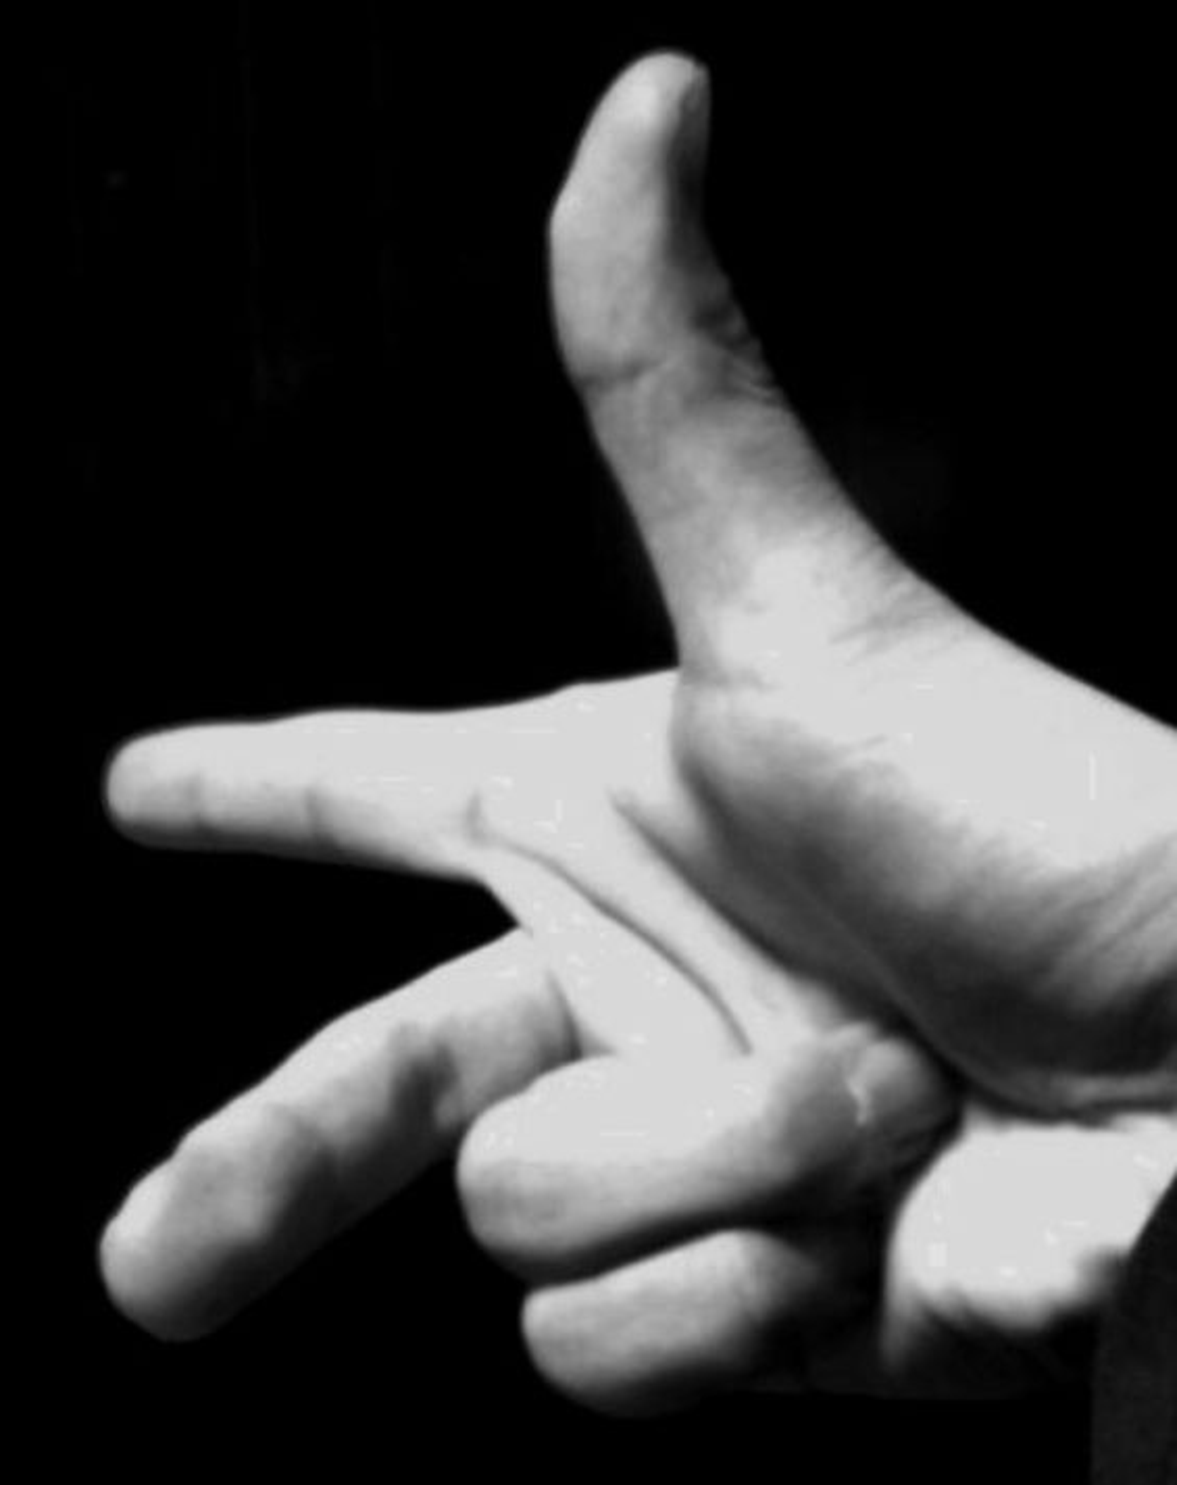
\includegraphics[keepaspectratio, width=3cm,height=3.75cm,clip]{migitekei_TE_mono_x.pdf}

                                    (a) 私の右手
                                    \label{fig:migitekei_TE_mono_x}
                                \end{center}
                            \end{minipage}
                            \begin{minipage}{0.5\hsize}
                                \begin{center}
                                    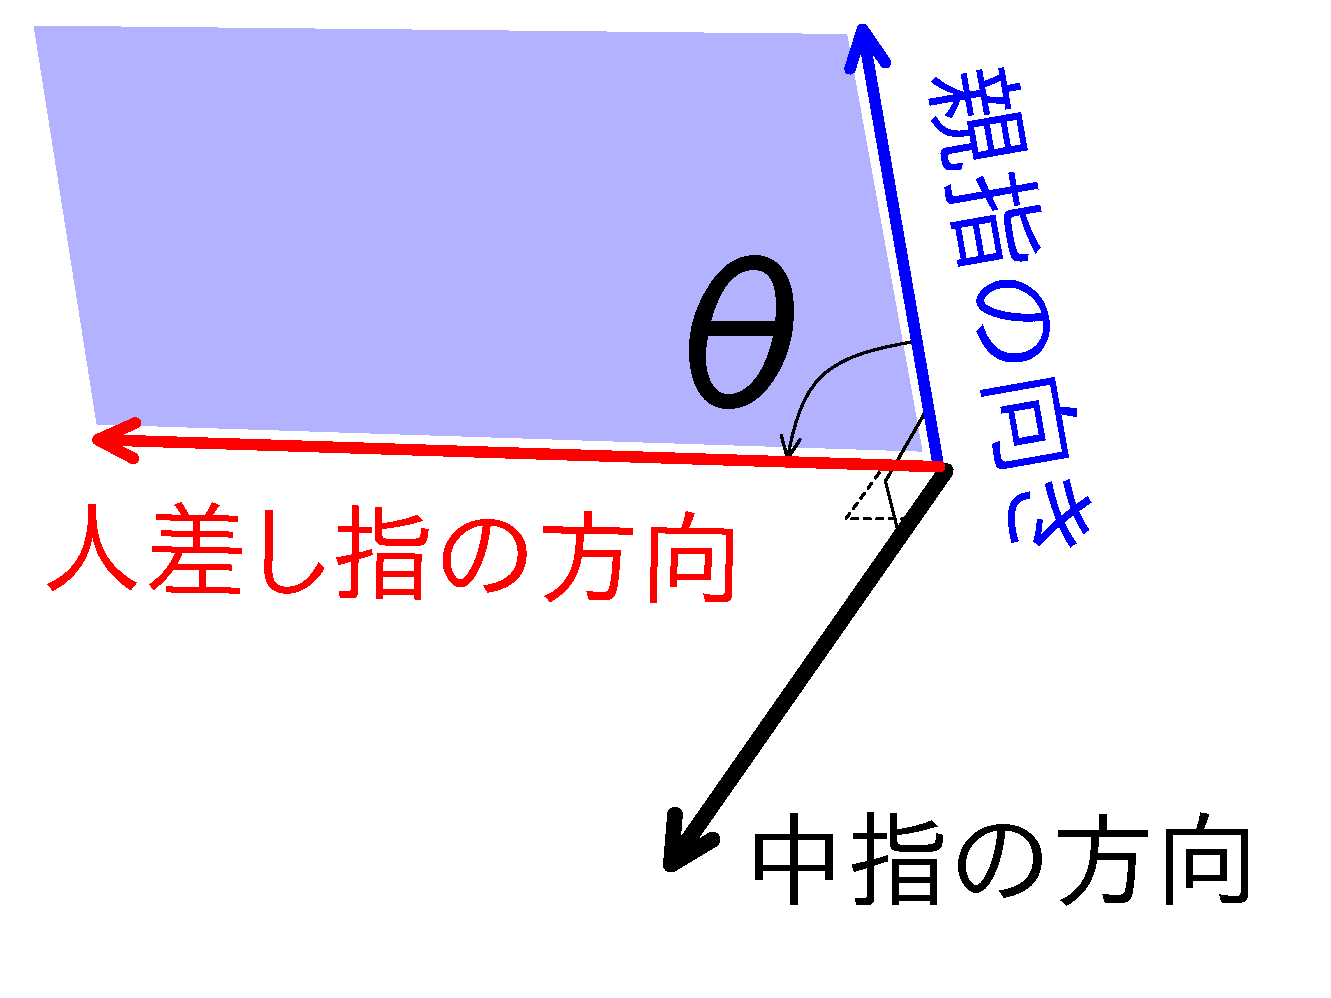
\includegraphics[keepaspectratio, width=3cm,height=3.75cm,clip]{migineji_Myhand.pdf}

                                    (b) 対応図
                                    \label{fig:migineji_Myhand}
                                \end{center}
                            \end{minipage}
                        \end{tabular}
                        \caption{右手系}
                    \end{figure}

                    \begin{figure}[hbt]
                        \begin{center}
                            \includegraphicslarge{VecKagenjoujo.pdf}
                            \caption{ベクトルの和$\cdot$差/$\cdot$積(内積/外積)}
                            \label{fig:VecKagenjoujo}
                        \end{center}
                    \end{figure}
                \end{memo}
